\documentclass[pdftex, unicode, a4paper,12pt,oneside,utf8x, usehyperref]{report-gost}
\usepackage[pdftex]{graphicx}
\usepackage{wrapfig}
\usepackage{floatflt}


\begin{document}
\title{Примеры решения задач симплекс-методом}
\author{Roman O Tsisyck}
\thispagestyle{empty}
\begin{center}
\vspace{8cm}
\end{center}

\begin{figure}[ht]
\centering
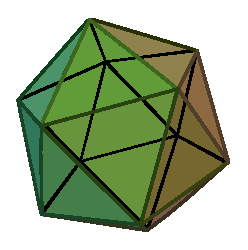
\includegraphics[width=0.8\textwidth]{img/simplex}
\end{figure}

\begin{center}
\LARGE{Simplex Solver} \\
\vspace{1cm}

\end{center}

\vspace{4cm}

\begin{center}
Цисык Р.О.\\
\end{center}

\vspace{\fill}

\begin{center}
\Large{г. Барнаул, 2009}
\end{center}

\clearpage
\newpage
\thispagestyle{empty}
\begin{center}
\ \vspace\fill
\end{center}


© 2009, Роман Цисык.
Версия документа 1.0 от 25 мая 2009 г. для SimpleSolver версии 1.0.

SimplexSolver представляет собой свободное программное обеспечение.
Вы можете свободно распространять и/или изменять программу при соблюдении условий лицензии \href{http://www.gnu.org/licenses/gpl.html}{GNU General Public License}
(версии 3 или более поздней), опубликованной
\href{http://www.fsf.org/}{Фондом свободного программного обеспечения.}
Данная программа распространяется в надежде, что она будет полезной,
но без всякой гарантии, в том числе без связанной гарантии товарной пригодности
или пригодности для частного использования.

Данная документация и логотип программы распространяется на условиях лицензии \href{http://www.creativecommons.org/licenses/by-sa/3.0/}{Creative Commons Attribution ShareAlike 3.0}.
Вы можете без ограничений распространять их, изменять и использовать в любых (в том числе коммерческих) целях при условии указания оригинального авторства и сохранения данной лицензии в производных работах.

\newpage

\chapter{Примеры решения задач}
\section{Пример I}

\renewcommand{\labelenumi}{\arabic{enumi})}
Задана ЗЛП с целевой функцией:
\begin{equation}
	F(\vec{X}) = x_1+x_2 \to max.
\end{equation}

Система ограничений имеет следующий вид:
\begin{equation}
\begin{cases}
20x_1+10x_2 \le 45\\
2x_1+7x_2 \le 14\\
x_i \ge 0 \\
\end{cases}
\end{equation}.

\subsection{Решение исходной ЗЛП}
Введем балансовые переменные и приведем к каноническому виду.
Для нахождения максимума, умножим целевую функцию на -1.

$$-F(\vec{X}) = -(-x_1-x_2) \to max$$
\begin{equation}
\begin{cases}
20x_1+10x_2+x_3=45\\
2x_1+7x_2+x_4=14\\
x_i, s_i \ge 0 \\
\end{cases}
\end{equation}

Составим таблицу и решим задачу симплекс-методом.

\begin{center}
\begin{tabular*}{\textwidth}{@{\extracolsep{\fill}}|c|c|c|c|c|c|c|c|c|}
\hline
$i$ & Базис & $C_i$ & B & $C_1 = -1$ & $C_2 = -1$ & $C_3 = 0$ & $C_4 = 0$ & $\Theta_i$ \\
\hline
$1$ & $P_3$ & $0$ & $45$ & $20$ & $10$ & $1$ & $0$ & $2,25$\\
$2$ & $P_4$ & $0$ & $14$ & $2$ & $7$ & $0$ & $1$ & $7$\\
\hline
$m+1$ & ~ & ~ & $0$ & $1$ & $1$ & $0$ & $0$ & ~ \\
\hline
\end{tabular*}
\end{center}
\begin{center}
\begin{tabular*}{\textwidth}{@{\extracolsep{\fill}}|c|c|c|c|c|c|c|c|c|}
\hline
$i$ & Базис & $C_i$ & B & $C_1 = -1$ & $C_2 = -1$ & $C_3 = 0$ & $C_4 = 0$ & $\Theta_i$ \\
\hline
$1$ & $P_1$ & $-1$ & $2,25$ & $1$ & $0,5$ & $0,05$ & $0$ & $4,5$\\
$2$ & $P_4$ & $0$ & $9,5$ & $0$ & $6$ & $-0,1$ & $1$ & $1,583$\\
\hline
$m+1$ & ~ & ~ & $-2,25$ & $0$ & $0,5$ & $-0,05$ & $0$ & ~ \\
\hline
\end{tabular*}
\end{center}
\begin{center}
\begin{tabular*}{\textwidth}{@{\extracolsep{\fill}}|c|c|c|c|c|c|c|c|c|}
\hline
$i$ & Базис & $C_i$ & B & $C_1 = -1$ & $C_2 = -1$ & $C_3 = 0$ & $C_4 = 0$ & $\Theta_i$ \\
\hline
$1$ & $P_1$ & $-1$ & $1,458$ & $1$ & $0$ & $0,05833$ & $-0,08333$ & $4,5$\\
$2$ & $P_2$ & $-1$ & $1,583$ & $0$ & $1$ & $-0,01667$ & $0,1667$ & $1,583$\\
\hline
$m+1$ & ~ & ~ & $-3,042$ & $0$ & $0$ & $-0,04167$ & $-0,08333$ & ~ \\
$m+1$ & ~ & ~ & $3,042$ & $0$ & $0$ & $0,04167$ & $0,08333$ & ~ \\
\hline
\end{tabular*}
\end{center}
Получен оптимальный план: $X^{опт} = (1,458;1,583)$, и оптимальное значение целевой функции $F^{опт} = 3,04$.

Тогда оптимальный план и значение двойственной симметричной ЗЛП:
\begin{align*}
	Y^{опт} = (0,042; 0,083),&~ Z^{опт} = 3,04.
\end{align*}

\begin{figure}[ht]
\centering
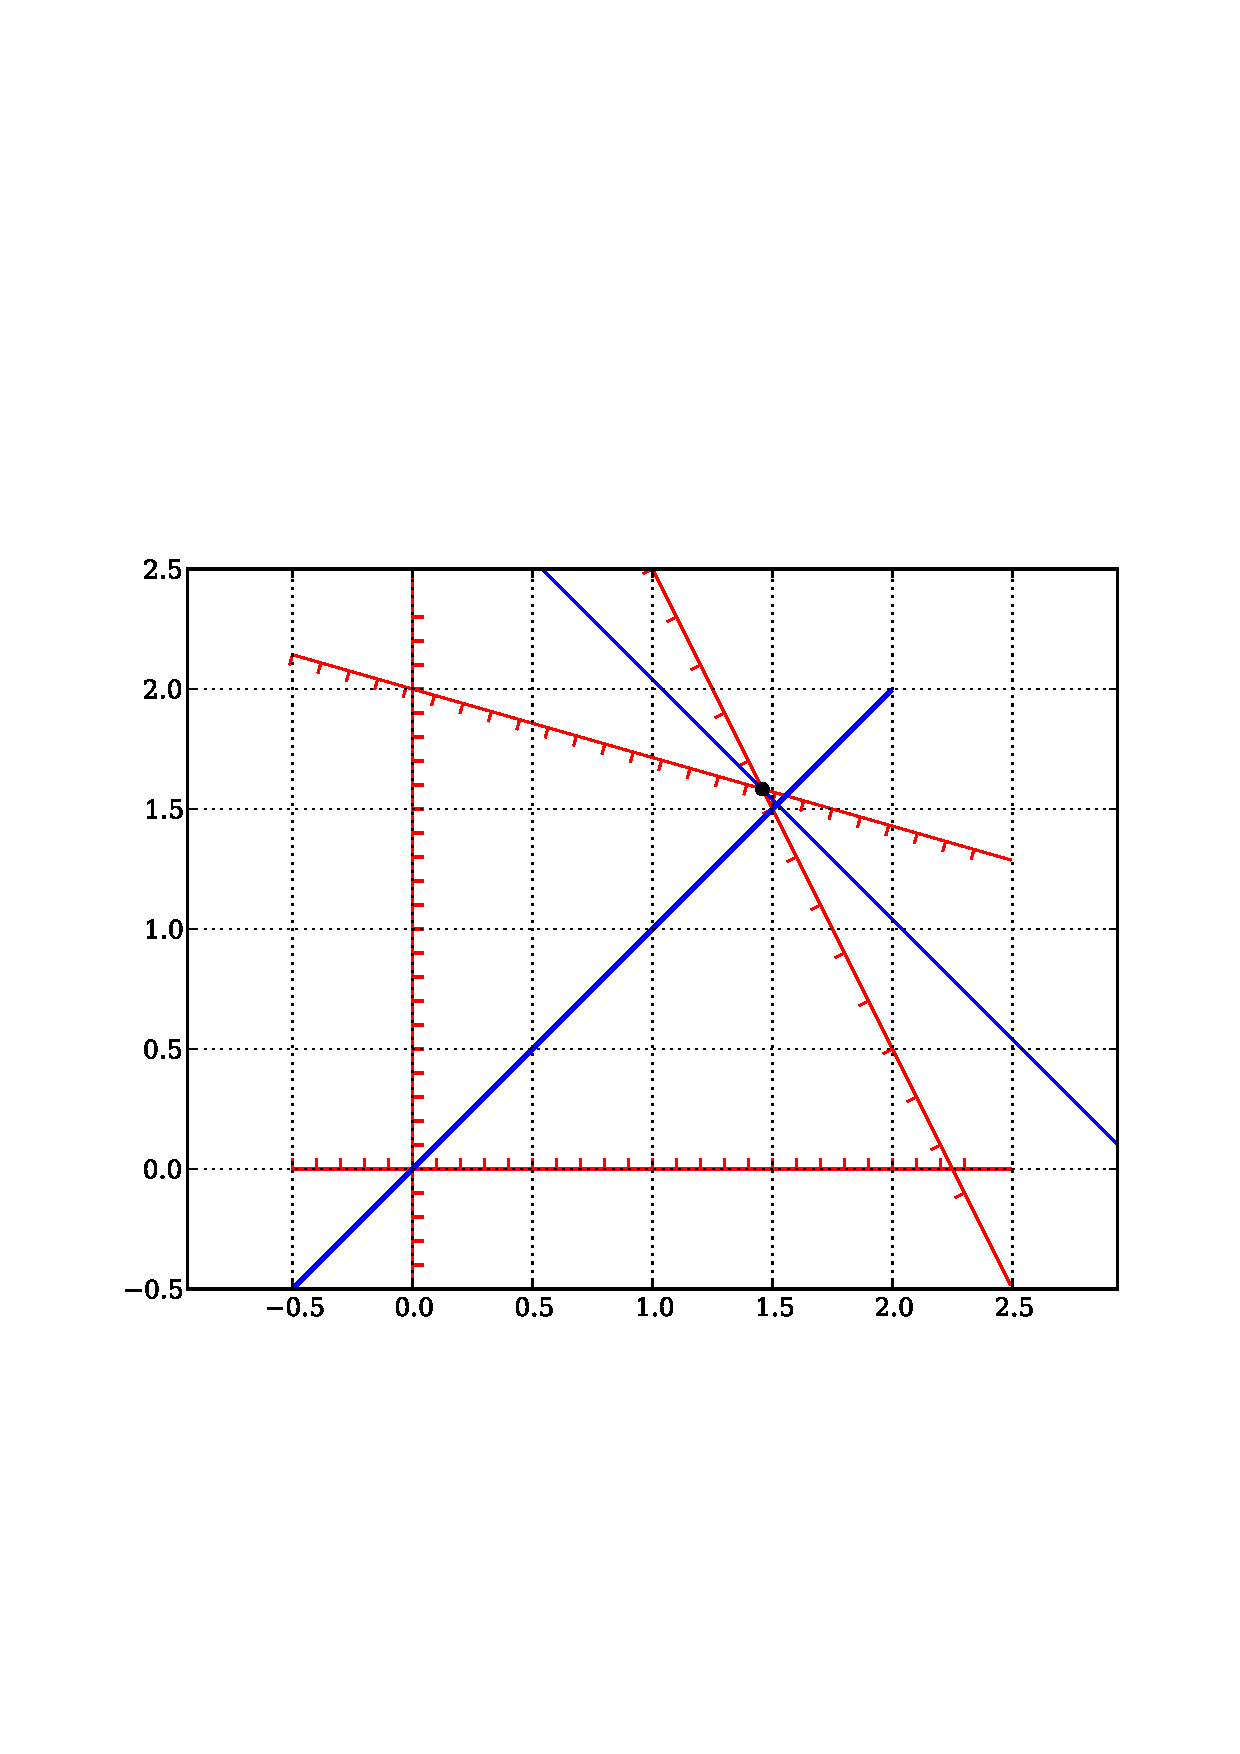
\includegraphics[width=\textwidth]{img/11}
\caption{Решение исходной ЗЛП графическим методом}
\end{figure}

\subsection{Решение двойственной ЗЛП}
Построим двойственную симметричную ЗЛП:

\begin{equation}
	Z(\vec{Y}) = 45 y_1 + 14y_2 \to min,
\end{equation}

\begin{equation}
\begin{cases}
20y_1 + 2y_2 \ge 1, \\
10y_1 + 7y_2 \ge 1, \\
y_1, y_2 \ge 0. \\
\end{cases}
\end{equation}

Введем искусственные переменные и приведем к каноническому виду.
\begin{equation}
	Z(\vec{Y}) = 45y_1+14y_2+Wy_5+Wy_6 \to min
\end{equation}

\begin{equation}
\begin{cases}
20y_1+2y_2-y_3+ s_5=1\\
10y_1+7y_2-y_4+ s_6=1\\
y_i, s_i \ge 0 \\
\end{cases}
\end{equation}
\begin{center}
\begin{tabular*}{\textwidth}{@{\extracolsep{\fill}}|c|c|c|c|c|c|c|c|c|c|c|}
\hline
$i$ & Базис & $B_i$ & C & $B_1 = 45$ & $B_2 = 14$ & $B_3 = 0$ & $B_4 = 0$ & $B_5 = W$ & $B_6 = W$ & $\Theta_i$ \\
\hline
$1$ & $P_5$ & W & $1$ & $20$ & $2$ & $-1$ & $0$ & $1$ & $0$ & $0,05$\\
$2$ & $P_6$ & W & $1$ & $10$ & $7$ & $0$ & $-1$ & $0$ & $1$ & $0,1$\\
\hline
$m+1$ & ~ & ~ & $0$ & $-45$ & $-14$ & $0$ & $0$ & $0$ & $0$ & ~ \\
\hline
$m+2$ & ~ & ~ & $2W$ & $30W$ & $9W$ & $-1W$ & $-1W$ & $0W$ & $0W$ & ~ \\
\hline
\end{tabular*}
\end{center}
\begin{center}
\begin{tabular*}{\textwidth}{@{\extracolsep{\fill}}|c|c|c|c|c|c|c|c|c|c|c|}
\hline
$i$ & Базис & $B_i$ & C & $B_1 = 45$ & $B_2 = 14$ & $B_3 = 0$ & $B_4 = 0$ & $B_5 = W$ & $B_6 = W$ & $\Theta_i$ \\
\hline
$1$ & $P_1$ & $45$ & $0,05$ & $1$ & $0,1$ & $-0,05$ & $0$ & $0,05$ & $0$ & $0,5$\\
$2$ & $P_6$ & W & $0,5$ & $0$ & $6$ & $0,5$ & $-1$ & $-0,5$ & $1$ & $0,08333$\\
\hline
$m+1$ & ~ & ~ & $2,25$ & $0$ & $-9,5$ & $-2,25$ & $0$ & $2,25$ & $0$ & ~ \\
\hline
$m+2$ & ~ & ~ & $0,5W$ & $0W$ & $6W$ & $0,5W$ & $-1W$ & $-1,5W$ & $0W$ & ~ \\
\hline
\end{tabular*}
\end{center}
\begin{center}
\begin{tabular*}{\textwidth}{@{\extracolsep{\fill}}|c|c|c|c|c|c|c|c|c|c|c|}
\hline
$i$ & Базис & $B_i$ & C & $B_1 = 45$ & $B_2 = 14$ & $B_3 = 0$ & $B_4 = 0$ & $B_5 = W$ & $B_6 = W$ & $\Theta_i$ \\
\hline
$1$ & $P_1$ & $45$ & $0,04167$ & $1$ & $0$ & $-0,05833$ & $0,01667$ & $0,05833$ & $-0,01667$ & ~\\
$2$ & $P_2$ & $14$ & $0,08333$ & $0$ & $1$ & $0,08333$ & $-0,1667$ & $-0,08333$ & $0,1667$ & ~\\
\hline
~ & ~ & ~ & $3,042$ & $0$ & $0$ & $-1,458$ & $-1,583$ & $1,458$ & $1,583$ & ~ \\
\hline
~ & ~ & ~ & $0W$ & $0W$ & $0W$ & $0W$ & $0W$ & $-1W$ & $-1W$ & ~ \\
\hline
\end{tabular*}
\end{center}
Получен оптимальный план: $Y^{опт} = (0,0417;0,0833)$, и оптимальное значение целевой функции $Z^{опт} = 3,04$.
\clearpage
\begin{figure}[ht]
\centering
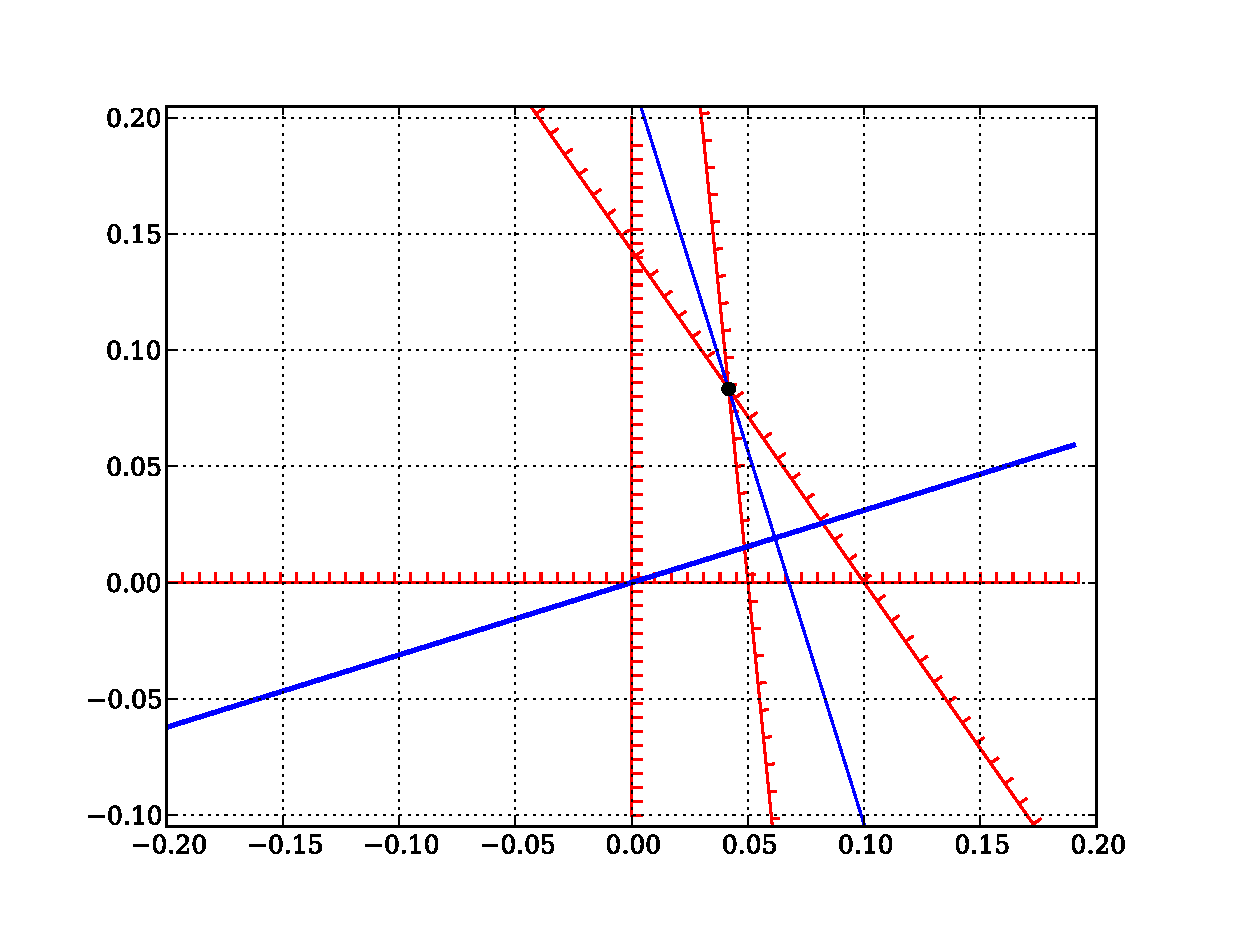
\includegraphics[width=0.9\textwidth]{img/12}
\caption{Решение двойственной задачи графическим методом}
\end{figure}

\subsection{Решение исходной и двойственное ЗЛП в программе}
Введем исходную и двойственную ЗЛП в программу и сравним результаты.

\begin{figure}[hb]
\centering
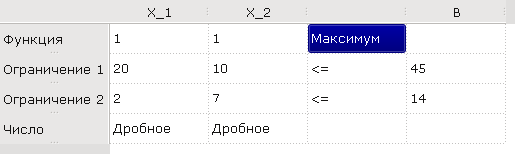
\includegraphics[scale=1.0]{img/problem11.png}
\caption{Условие задачи в программе}
\end{figure}
\newpage
\clearpage

\begin{figure}[ht]
\centering
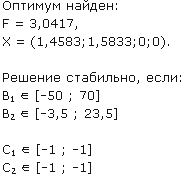
\includegraphics[scale=1.0]{img/solution11.png}
\caption{Решение задачи в программе}
\end{figure}

\begin{figure}[ht]
\centering
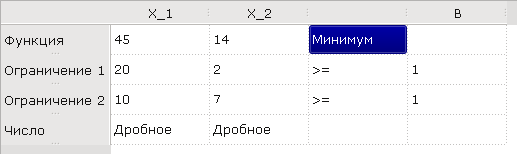
\includegraphics[scale=1.0]{img/problem12.png}
\caption{Условие двойственной задачи в программе}
\end{figure}

\begin{figure}[ht]
\centering
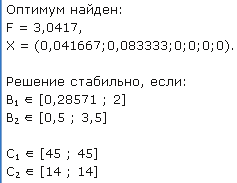
\includegraphics[scale=1.0]{img/solution12.png}
\caption{Решение двойственной задачи в программе}
\end{figure}

\clearpage

\section{Пример II}

\subsection{Постановка задачи}
\renewcommand{\labelenumi}{\arabic{enumi})}
Задана ЗЛП в каноническом виде:
\begin{equation}
	F(\vec{X}) = 2x_1 - 5x_2 - x_3 + x_4 \to max,
\end{equation}

\begin{equation}
\begin{cases}
x_1 + 3x_2 - x_3 + x_4 = 1 \\
2x_1 + 3x_3 - x_4 = 2 \\
x_1, x_2, x_3, x_4 \ge 0
\end{cases}
\end{equation}.

Необходимо:
\begin{enumerate}
\item Решить исходную ЗЛП методом искусственного базиса;
\item Решить исходную ЗЛП графически;
\end{enumerate}

\subsection{Решение исходной ЗЛП методом искусственного базиса}
Введем искусственные переменные и приведем к каноническому виду.
Для нахождения максимума, умножим целевую функцию на -1.
Заметим, что вектор во втором столбце уже является
единичным после деления строки на 3.

$$-F(\vec{X}) = -(-2x_1+5x_2+x_3-x_4+Wx_5) \to max$$
\begin{equation}
\label{cannonical}
\begin{cases}
\frac{1}{3} x_1+x_2 - \frac{1}{3} x_3 + \frac{1}{3} x_4=\frac{1}{3} \\
2x_1+3x_3-x_4+ s_5=2\\
x_i, s_i \ge 0 \\
\end{cases}
\end{equation}

\begin{center}
\begin{tabular*}{\textwidth}{@{\extracolsep{\fill}}|c|c|c|c|c|c|c|c|c|c|}
\hline
$i$ & Базис & $C_i$ & B & $C_1 = -2$ & $C_2 = 5$ & $C_3 = 1$ & $C_4 = -1$ & $C_5 = W$ & $\Theta_i$ \\
\hline
$1$ & $P_2$ & $5$ & $0,3333$ & $0,3333$ & $1$ & $-0,3333$ & $0,3333$ & $0$ & --\\
$2$ & $P_5$ & W & $2$ & $2$ & $0$ & $3$ & $-1$ & $1$ & $0,6667$\\
\hline
$m+1$ & ~ & ~ & $1,667$ & $3,667$ & $0$ & $-2,667$ & $2,667$ & $0$ & ~ \\
\hline
$m+2$ & ~ & ~ & $2W$ & $2W$ & $0W$ & $3W$ & $-1W$ & $0W$ & ~ \\
\hline
\end{tabular*}
\end{center}
\begin{center}
\begin{tabular*}{\textwidth}{@{\extracolsep{\fill}}|c|c|c|c|c|c|c|c|c|c|}
\hline
$i$ & Базис & $C_i$ & B & $C_1 = -2$ & $C_2 = 5$ & $C_3 = 1$ & $C_4 = -1$ & $C_5 = W$ & $\Theta_i$ \\
\hline
$1$ & $P_2$ & $5$ & $0,5556$ & $0,5556$ & $1$ & $0$ & $0,2222$ & $0,1111$ & $1$\\
$2$ & $P_3$ & $1$ & $0,6667$ & $0,6667$ & $0$ & $1$ & $-0,3333$ & $0,3333$ & $1$\\
\hline
$m+1$ & ~ & ~ & $3,444$ & $5,444$ & $0$ & $0$ & $1,778$ & $0,8889$ & ~ \\
\hline
$m+2$ & ~ & ~ & $0W$ & $0W$ & $0W$ & $0W$ & $0W$ & $-1W$ & ~ \\
\hline
\end{tabular*}
\end{center}
\begin{center}
\begin{tabular*}{\textwidth}{@{\extracolsep{\fill}}|c|c|c|c|c|c|c|c|c|c|}
\hline
$i$ & Базис & $C_i$ & B & $C_1 = -2$ & $C_2 = 5$ & $C_3 = 1$ & $C_4 = -1$ & $C_5 = W$ & $\Theta_i$ \\
\hline
$1$ & $P_1$ & $-2$ & $1$ & $1$ & $1,8$ & $0$ & $0,4$ & $0,2$ & $1$\\
$2$ & $P_3$ & $1$ & $0$ & $0$ & $-1,2$ & $1$ & $-0,6$ & $0,2$ & $1$\\
\hline
$m+1$ & ~ & ~ & $-2$ & $0$ & $-9,8$ & $0$ & $-0,4$ & $-0,2$ & ~ \\
\hline
$m+2$ & ~ & ~ & $0W$ & $0W$ & $0W$ & $0W$ & $0W$ & $-1W$ & ~ \\
\hline
\end{tabular*}
\end{center}
Получен оптимальный план: $X^{опт} = (1;0;0;0;0)$,
и оптимальное значение целевой функции $F^{опт} = 2$.

\subsection{Решение исходной ЗЛП графическим методом}
\begin{figure}[ht]
\centering
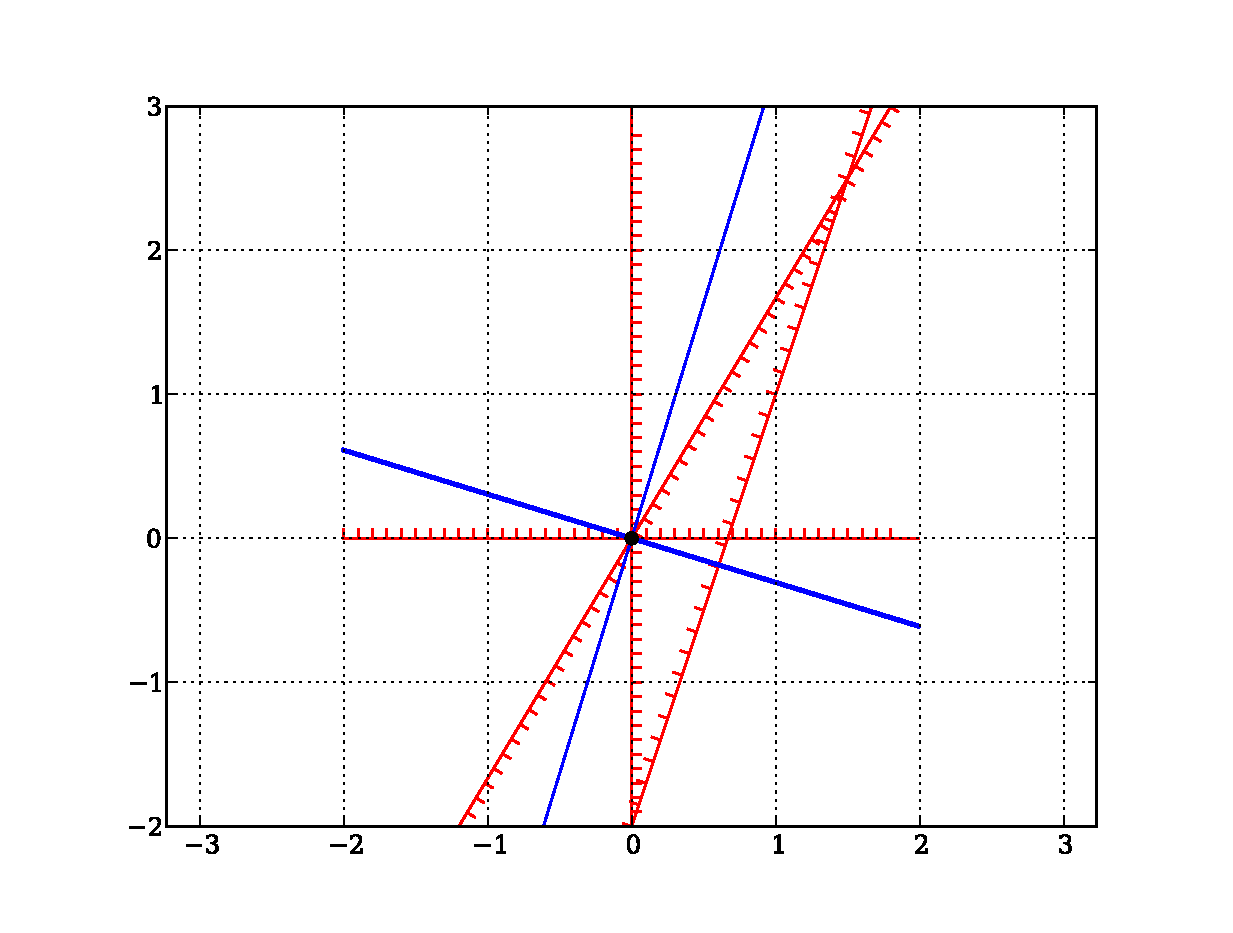
\includegraphics[width=\textwidth]{img/21}
\caption{Решение графическим методом}\label{21}
\end{figure}
\section{Пример III}
Задана ЗЛП:
$$F(\vec{X}) = x_1+4x_2 \to max$$
\begin{equation}
\label{system}
\begin{cases}
2x_1+4x_2 \le 17\\
10x_1+3x_2 \le 15\\
x_i \ge 0 \\
\end{cases}
\end{equation}

\subsection{Решение исходной ЗЛП}
Введем искусственные переменные и приведем к каноническому виду.
Для нахождения максимума, умножим целевую функцию на -1.

$$-F(\vec{X}) = -(-x_1-4x_2) \to max$$
\begin{equation}
\label{cannonical}
\begin{cases}
2x_1+4x_2+x_3=17\\
10x_1+3x_2+x_4=15\\
x_i, s_i \ge 0 \\
\end{cases}
\end{equation}

\begin{center}
\begin{tabular*}{\textwidth}{@{\extracolsep{\fill}}|c|c|c|c|c|c|c|c|c|}
\hline
$i$ & Базис & $C_i$ & B & $C_1 = -1$ & $C_2 = -4$ & $C_3 = 0$ & $C_4 = 0$ & $\Theta_i$ \\
\hline
$1$ & $P_3$ & $0$ & $17$ & $2$ & $4$ & $1$ & $0$ & $4,25$\\
$2$ & $P_4$ & $0$ & $15$ & $10$ & $3$ & $0$ & $1$ & $5$\\
\hline
$m+1$ & ~ & ~ & $0$ & $1$ & $4$ & $0$ & $0$ & ~ \\
\hline
\end{tabular*}
\end{center}
\begin{center}
\begin{tabular*}{\textwidth}{@{\extracolsep{\fill}}|c|c|c|c|c|c|c|c|c|}
\hline
$i$ & Базис & $C_i$ & B & $C_1 = -1$ & $C_2 = -4$ & $C_3 = 0$ & $C_4 = 0$ & $\Theta_i$ \\
\hline
$1$ & $P_2$ & $-4$ & $4,25$ & $0,5$ & $1$ & $0,25$ & $0$ & $4,25$\\
$2$ & $P_4$ & $0$ & $2,25$ & $8,5$ & $0$ & $-0,75$ & $1$ & $5$\\
\hline
$m+1$ & ~ & ~ & $-17$ & $0$ & $0$ & $-1$ & $0$ & ~ \\
\hline
\end{tabular*}
\end{center}
Получен оптимальный план: $X^{опт} = (0;4,25)$, и оптимальное значение целевой функции $F^{опт} = 17$.

\subsection{Нахождение целочисленных решений}
Компонент $P_2$ полученного плана не является целочисленным. Применим алгоритм Гомори.
Первое отсечение:
\begin{equation}
-0,5 x_1 - 0,25 x_3 + U_1 = -0,25.
\end{equation}
\begin{center}
\begin{tabular*}{\textwidth}{@{\extracolsep{\fill}}|c|c|c|c|c|c|c|c|c|c|}
\hline
$i$ & Базис & $C_i$ & B & $C_1 = -1$ & $C_2 = -4$ & $C_3 = 0$ & $C_4 = 0$ & $C_5 = 0$ & $\Theta_i$ \\
\hline
$1$ & $P_2$ & $-4$ & $4,25$ & $0,5$ & $1$ & $0,25$ & $0$ & $0$ & --\\
$2$ & $P_4$ & $0$ & $2,25$ & $8,5$ & $0$ & $-0,75$ & $1$ & $0$ & --\\
$3$ & $P_5$ & $0$ & $-0,25$ & $-0,5$ & $0$ & $-0,25$ & $0$ & $1$ & --\\
\hline
$m+1$ & ~ & ~ & $-17$ & $0$ & $0$ & $0$ & $0$ & $0$ & ~ \\
\hline
\end{tabular*}
\end{center}
\begin{center}
\begin{tabular*}{\textwidth}{@{\extracolsep{\fill}}|c|c|c|c|c|c|c|c|c|c|}
\hline
$i$ & Базис & $C_i$ & B & $C_1 = -1$ & $C_2 = -4$ & $C_3 = 0$ & $C_4 = 0$ & $C_5 = 0$ & $\Theta_i$ \\
\hline
$1$ & $P_2$ & $-4$ & $4$ & $0$ & $1$ & $0$ & $0$ & $1$ & --\\
$2$ & $P_4$ & $0$ & $-2$ & $0$ & $0$ & $-5$ & $1$ & $17$ & --\\
$3$ & $P_1$ & $-1$ & $0,5$ & $1$ & $0$ & $0,5$ & $0$ & $-2$ & --\\
\hline
$m+1$ & ~ & ~ & $-17$ & $0$ & $0$ & $0$ & $0$ & $0$ & ~ \\
\hline
\end{tabular*}
\end{center}
Второе отсечение:
\begin{equation}
- 0,5 x_3  + U_2 = -0,5.
\end{equation}
\begin{center}
\begin{tabular*}{\textwidth}{@{\extracolsep{\fill}}|c|c|c|c|c|c|c|c|c|c|c|}
\hline
$i$ & Базис & $C_i$ & B & $C_1 = -1$ & $C_2 = -4$ & $C_3 = 0$ & $C_4 = 0$ & $C_5 = 0$ & $C_6 = 0$ & $\Theta_i$ \\
\hline
$1$ & $P_2$ & $-4$ & $4$ & $0$ & $1$ & $0$ & $0$ & $1$ & $0$ & --\\
$2$ & $P_4$ & $0$ & $-2$ & $0$ & $0$ & $-5$ & $1$ & $17$ & $0$ & --\\
$3$ & $P_1$ & $-1$ & $0,5$ & $1$ & $0$ & $0,5$ & $0$ & $-2$ & $0$ & --\\
$4$ & $P_6$ & $0$ & $-0,5$ & $0$ & $0$ & $-0,5$ & $0$ & $0$ & $1$ & --\\
\hline
$m+1$ & ~ & ~ & $-17$ & $0$ & $0$ & $0$ & $0$ & $0$ & $0$ & ~ \\
\hline
\end{tabular*}
\end{center}
\begin{center}
\begin{tabular*}{\textwidth}{@{\extracolsep{\fill}}|c|c|c|c|c|c|c|c|c|c|c|}
\hline
$i$ & Базис & $C_i$ & B & $C_1 = -1$ & $C_2 = -4$ & $C_3 = 0$ & $C_4 = 0$ & $C_5 = 0$ & $C_6 = 0$ & $\Theta_i$ \\
\hline
$1$ & $P_2$ & $-4$ & $4$ & $0$ & $1$ & $0$ & $0$ & $1$ & $0$ & --\\
$2$ & $P_4$ & $0$ & $3$ & $0$ & $0$ & $0$ & $1$ & $17$ & $-10$ & --\\
$3$ & $P_1$ & $-1$ & $0$ & $1$ & $0$ & $0$ & $0$ & $-2$ & $1$ & --\\
$4$ & $P_3$ & $0$ & $1$ & $0$ & $0$ & $1$ & $0$ & $0$ & $-2$ & --\\
\hline
$m+1$ & ~ & ~ & $-17$ & $0$ & $0$ & $0$ & $0$ & $0$ & $0$ & ~ \\
\hline
\end{tabular*}
\end{center}
Получен оптимальный план: $X^{опт} = (0;4)$, и оптимальное значение целевой функции $F^{опт} = 16$.

\newpage
\subsection{Решение ЗЛП в программе}
Введем ЗЛП в программу и сравним результаты.

\begin{figure}[hb]
\centering
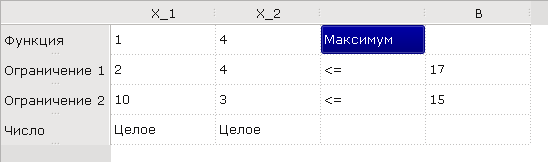
\includegraphics[scale=1.0]{img/problem31.png}
\caption{Условие задачи в программе}
\end{figure}

\begin{figure}[ht]
\centering
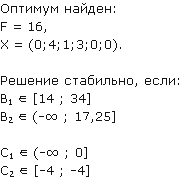
\includegraphics[scale=1.0]{img/solution31.png}
\caption{Решение задачи в программе}
\end{figure}

\section{Пример IV}

\subsection{Постановка задачи}
\renewcommand{\labelenumi}{\arabic{enumi})}
Задана ЗЛП:
$$F(\vec{X}) = x_1+4x_2 \to max$$
\begin{equation}
\label{system}
\begin{cases}
2x_1+4x_2 \le 17\\
10x_1+3x_2 \le 15\\
x_i \ge 0 \\
\end{cases}
\end{equation}

Необходимо:
\begin{enumerate}
\item Привести исходную ЗЛП к каноническому виду и решить методом искусственного базиса;
\item Найти целочисленное решение, используя алгоритм Гомори.
\end{enumerate}

\subsection{Решение исходной ЗЛП методом искусственного базиса}
Введем искусственные переменные и приведем к каноническому виду.
Для нахождения максимума, умножим целевую функцию на -1.

$$-F(\vec{X}) = -(-x_1-4x_2) \to max$$
\begin{equation}
\label{cannonical}
\begin{cases}
2x_1+4x_2+x_3=17\\
10x_1+3x_2+x_4=15\\
x_i, s_i \ge 0 \\
\end{cases}
\end{equation}

\begin{center}
\begin{tabular*}{\textwidth}{@{\extracolsep{\fill}}|c|c|c|c|c|c|c|c|c|}
\hline
$i$ & Базис & $C_i$ & B & $C_1 = -1$ & $C_2 = -4$ & $C_3 = 0$ & $C_4 = 0$ & $\Theta_i$ \\
\hline
$1$ & $P_3$ & $0$ & $17$ & $2$ & $4$ & $1$ & $0$ & $4,25$\\
$2$ & $P_4$ & $0$ & $15$ & $10$ & $3$ & $0$ & $1$ & $5$\\
\hline
$m+1$ & ~ & ~ & $0$ & $1$ & $4$ & $0$ & $0$ & ~ \\
\hline
\end{tabular*}
\end{center}
\begin{center}
\begin{tabular*}{\textwidth}{@{\extracolsep{\fill}}|c|c|c|c|c|c|c|c|c|}
\hline
$i$ & Базис & $C_i$ & B & $C_1 = -1$ & $C_2 = -4$ & $C_3 = 0$ & $C_4 = 0$ & $\Theta_i$ \\
\hline
$1$ & $P_2$ & $-4$ & $4,25$ & $0,5$ & $1$ & $0,25$ & $0$ & $4,25$\\
$2$ & $P_4$ & $0$ & $2,25$ & $8,5$ & $0$ & $-0,75$ & $1$ & $5$\\
\hline
$m+1$ & ~ & ~ & $-17$ & $0$ & $0$ & $-1$ & $0$ & ~ \\
\hline
\end{tabular*}
\end{center}
Получен оптимальный план: $X^{опт} = (0;4,25)$, и оптимальное значение целевой функции $F^{опт} = 17$.

\subsection{Нахождение целочисленных решений}
Компонент $P_2$ полученного плана не является целочисленным. Применим алгоритм Гомори.
Первое отсечение:
\begin{equation}
-0,5 x_1 - 0,25 x_3 + U_1 = -0,25.
\end{equation}
\begin{center}
\begin{tabular*}{\textwidth}{@{\extracolsep{\fill}}|c|c|c|c|c|c|c|c|c|c|}
\hline
$i$ & Базис & $C_i$ & B & $C_1 = -1$ & $C_2 = -4$ & $C_3 = 0$ & $C_4 = 0$ & $C_5 = 0$ & $\Theta_i$ \\
\hline
$1$ & $P_2$ & $-4$ & $4,25$ & $0,5$ & $1$ & $0,25$ & $0$ & $0$ & --\\
$2$ & $P_4$ & $0$ & $2,25$ & $8,5$ & $0$ & $-0,75$ & $1$ & $0$ & --\\
$3$ & $P_5$ & $0$ & $-0,25$ & $-0,5$ & $0$ & $-0,25$ & $0$ & $1$ & --\\
\hline
$m+1$ & ~ & ~ & $-17$ & $0$ & $0$ & $0$ & $0$ & $0$ & ~ \\
\hline
\end{tabular*}
\end{center}
\begin{center}
\begin{tabular*}{\textwidth}{@{\extracolsep{\fill}}|c|c|c|c|c|c|c|c|c|c|}
\hline
$i$ & Базис & $C_i$ & B & $C_1 = -1$ & $C_2 = -4$ & $C_3 = 0$ & $C_4 = 0$ & $C_5 = 0$ & $\Theta_i$ \\
\hline
$1$ & $P_2$ & $-4$ & $4$ & $0$ & $1$ & $0$ & $0$ & $1$ & --\\
$2$ & $P_4$ & $0$ & $-2$ & $0$ & $0$ & $-5$ & $1$ & $17$ & --\\
$3$ & $P_1$ & $-1$ & $0,5$ & $1$ & $0$ & $0,5$ & $0$ & $-2$ & --\\
\hline
$m+1$ & ~ & ~ & $-17$ & $0$ & $0$ & $0$ & $0$ & $0$ & ~ \\
\hline
\end{tabular*}
\end{center}
Второе отсечение:
\begin{equation}
- 0,5 x_3  + U_2 = -0,5.
\end{equation}
\begin{center}
\begin{tabular*}{\textwidth}{@{\extracolsep{\fill}}|c|c|c|c|c|c|c|c|c|c|c|}
\hline
$i$ & Базис & $C_i$ & B & $C_1 = -1$ & $C_2 = -4$ & $C_3 = 0$ & $C_4 = 0$ & $C_5 = 0$ & $C_6 = 0$ & $\Theta_i$ \\
\hline
$1$ & $P_2$ & $-4$ & $4$ & $0$ & $1$ & $0$ & $0$ & $1$ & $0$ & --\\
$2$ & $P_4$ & $0$ & $-2$ & $0$ & $0$ & $-5$ & $1$ & $17$ & $0$ & --\\
$3$ & $P_1$ & $-1$ & $0,5$ & $1$ & $0$ & $0,5$ & $0$ & $-2$ & $0$ & --\\
$4$ & $P_6$ & $0$ & $-0,5$ & $0$ & $0$ & $-0,5$ & $0$ & $0$ & $1$ & --\\
\hline
$m+1$ & ~ & ~ & $-17$ & $0$ & $0$ & $0$ & $0$ & $0$ & $0$ & ~ \\
\hline
\end{tabular*}
\end{center}
\begin{center}
\begin{tabular*}{\textwidth}{@{\extracolsep{\fill}}|c|c|c|c|c|c|c|c|c|c|c|}
\hline
$i$ & Базис & $C_i$ & B & $C_1 = -1$ & $C_2 = -4$ & $C_3 = 0$ & $C_4 = 0$ & $C_5 = 0$ & $C_6 = 0$ & $\Theta_i$ \\
\hline
$1$ & $P_2$ & $-4$ & $4$ & $0$ & $1$ & $0$ & $0$ & $1$ & $0$ & --\\
$2$ & $P_4$ & $0$ & $3$ & $0$ & $0$ & $0$ & $1$ & $17$ & $-10$ & --\\
$3$ & $P_1$ & $-1$ & $0$ & $1$ & $0$ & $0$ & $0$ & $-2$ & $1$ & --\\
$4$ & $P_3$ & $0$ & $1$ & $0$ & $0$ & $1$ & $0$ & $0$ & $-2$ & --\\
\hline
$m+1$ & ~ & ~ & $-17$ & $0$ & $0$ & $0$ & $0$ & $0$ & $0$ & ~ \\
\hline
\end{tabular*}
\end{center}
Получен оптимальный план: $X^{опт} = (0;4)$, и оптимальное значение целевой функции $F^{опт} = 16$.



\end{document}
